\chapter{Marco teórico}

En aplicaciones y programas tradicionales, hay una diferenciación entre código confiable y entrada no confiable, por lo que hay muchas formas de protegerse contra el CSS o el SQL injection (consultas preparadas, comprobando el regex de la entrada, etc.). Sin embargo, en LLMs, las instrucciones de sistema y datos de usuario se integran en un mismo prompt y se procesan con el mismo mecanismo lingüístico \cite{gulyamov2026promptinjection}. Por este motivo técnicas como usar etiquetas o delimitadores de inicio y final de intrucción pueden ser anuladas por instrucciones escritas en lenguaje natural  \cite{gulyamov2026promptinjection}. Esta carencia de límites rígidos aumenta las posibilidades de ataque, sobre todo cuando el modelo tiene acceso a herramientas o consume contenido externo (como buscar en la web, etc.)

Un LLM no razona ni entiende las instrucciones escritas, sino que es un modelo estadístico que predice el siguiente token a partir del contexto \cite{ibm_llm_security}. Por ello la forma de atacar a estos sistemas es introduciendo instrucciones maliciosas (en lenguaje natural) dentro del contexto con el objetivo de alterar su comportamiento. Este ataque puede ser de forma directa o indirecta:

Se considera ataque por \textbf{inyección directa} cuando el adversario interactúa con el LLM e intenta inducir respuestas que normalmente estarían restringidas (jailbreaking). \cite{benjamin2024systematically} En la \textbf{inyección indirecta}, el contenido malicioso se introduce en fuentes externas que el sistema consume (web, documentos, repositorios, etc.) y el modelo lo interpreta como instrucciones, a menudo sin que el usuario lo advierta \cite{gulyamov2026promptinjection,greshake2023indirectpromptinjection}.

Según un estudio de la Unión Europea \cite{greshake2023indirectpromptinjection} los ataques a modelos de lenguaje siguen la siguiente taxonomía:

\begin{itemize}
	\item \textbf{Exfiltración de datos.} Exfiltración de datos.
	\item \textbf{Fraude y estafas.} Fishing, suplantación de identidad, etc.
	\item \textbf{Intrusión.} Aprovecha el modelo como puerta trasera para escalar privilegios.
	\item \textbf{Malware.} Los prompts pueden actuar como malware lógico y propagarse como gusanos entre aplicaciones.
	\item \textbf{Contenido manipulado.} Sesga resúmenes, oculta fuentes, propaga desinformación o publicidad encubierta.
	\item \textbf{Disponibilidad.} Provoca denegación de servicio (incrementando el cómputo mediante instrucciones costosas).
\end{itemize}

\section{Relación con seguridad clásica (CIA y STRIDE)}

Estos riesgos se pueden relacionar con los principios de seguridad clásica:

\begin{itemize}
	\item \textbf{Confidencialidad:} exfiltración de datos sensibles por respuestas del modelo o herramientas.
	\item \textbf{Integridad:} acciones para alterar datos, como generacion de sentencias maliciosas que alteren el contenido de la db.
	\item \textbf{Disponibilidad:} prompts que aumentan el coste computacional, bucles de herramientas o peticiones masivas.
\end{itemize}

Con STRIDE, los ataques se interpretan así:
\begin{itemize}
	\item \textbf{Spoofing:} el atacante se hace pasar por una fuente confiable (documento, sistema o rol) dentro del contexto.
	\item \textbf{Tampering:} alteración de datos mediante herramientas del modelo.
	\item \textbf{Repudiation:} ausencia de trazabilidad suficiente para atribuir el origen de una inyección.
	\item \textbf{Information Disclosure:} filtraciones de datos sensibles mediante respuestas del modelo.
	\item \textbf{Denial of Service:} tool-calling encadenado, o muchas consultas al modelo hasta que afecte su disponibilidad.
	\item \textbf{Elevation of Privilege:} uso indebido de herramientas para acceder a datos restringidos.
\end{itemize}

\newpage

\section{Matriz MITRE ATLAS}
MITRE ATLAS organiza tácticas y técnicas específicas para ataques contra sistemas que usan modelos de lenguaje\cite{mitre_atlas}. Esta es la matriz de amenazas relacionadas con la inteligenia artificial y los modelos de lenguaje:


\begin{figure}[H]
    \centering
    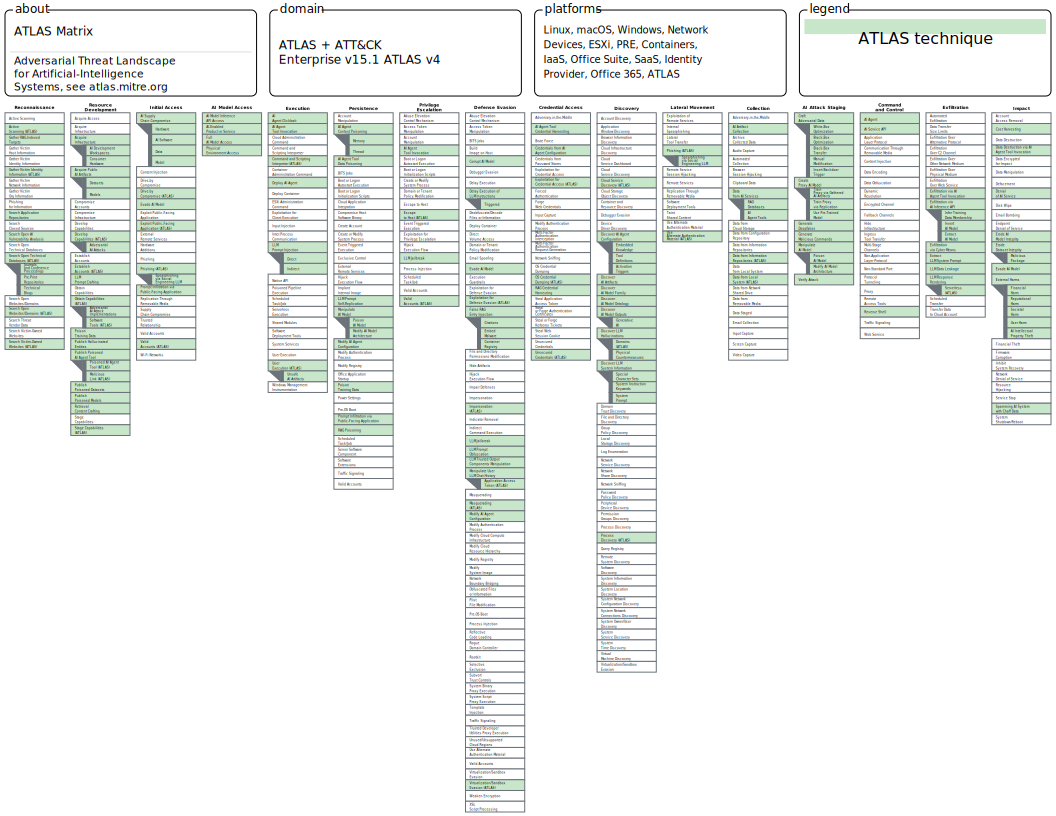
\includegraphics[width=1\linewidth]{Imagenes/ATLAS_Matrix.pdf}
    \caption{Matriz mitre de amenazas relacionadas con modelos de lenguaje}
    \label{fig:mitre-llms}
\end{figure}



En el contexto de este proyecto, relacionan los escenarios principales:

\begin{table}[H]
\centering
\begin{tabular}{|l|l|l|}
\hline
\textbf{Técnica} & \textbf{Táctica} & \textbf{ID} \\ \hline
Search Open AI Vulnerability Analysis & Reconnaissance & AML.T0001 \\ \hline
LLM Prompt Crafting & Resource Development & AML.T0065 \\ \hline
LLM Prompt Injection & Execution & AML.T0051 \\ \hline
Prompt Infiltration via Public-Facing Applcication & Initial Access, Persistence & AML.T0093 \\ \hline
%RAG Poisoning & Persistence & AML.T0070 \\ \hline
%AI Agent Tool Data Poisoning & Persistence & AML.T0099 \\ \hline
AI Agent Tool Invocation & Execution, Priv. Escalation & AML.T0053 \\ \hline
Data from AI Services & Collection & AML.T0085 \\ \hline
LLM Data Leakage & Exfiltration & AML.T0057 \\ \hline
Exfiltration via AI Agent Tool Invocation & Exfiltration & AML.T0086 \\ \hline
Denial of AI Service & Impact & AML.T0029 \\ \hline
Erode AI Model Integrity & Impact & AML.T0031 \\ \hline
\end{tabular}
\caption{Escenarios relacionados con el proyecto}
\label{tab:mitre-atlas-escenarios}
\end{table}




